\documentclass[aspectratio=169]{beamer}

% Custom theme and packages
\usepackage{beamertheme-custom}
% Custom symbols and commands
\usepackage{symbols-custom}

\usepackage{graphicx}
\graphicspath{{figures/}}

\title{Signal Detection Theory (SDT)}
\author{Joachim Vandekerckhove}
\date{Winter 2025}

\begin{document}

\maketitle

% \section{Signal Detection Theory (SDT)}

\begin{frame}{Core Idea: Decision in Noise}
  \frametitle{SDT: Core Idea}
  How do we make categorical judgments based on ambiguous or noisy information?
  \begin{itemize}
    \item Radiologist detecting a tumor
    \item Witness identifying a suspect
    \item Participant hearing a faint tone
  \end{itemize}
  \pause
  The challenge: Distinguishing target \emph{signal} from background \emph{noise}.
  \pause
  SDT formalizes the decision process into two components:
  \begin{enumerate}
    \item \textbf{Sensitivity:} How well can the system separate signal from noise? (Information quality)
    \item \textbf{Bias/Criterion:} What decision rule is used? (Strategy, goals, expectations)
  \end{enumerate}
  \pause
  Allows us to \emph{independently} quantify sensitivity and bias, unlike simple accuracy.
\end{frame}

\begin{frame}{Historical Roots}
  \frametitle{SDT: History \& Significance}
  Developed in 1950s/60s (Green, Swets, Tanner, Egan, ...).
  \pause
  Shift from classical \emph{threshold theories} (Fechner, Thurstone) which assumed fixed sensory thresholds.
  \pause

  SDT introduced a probabilistic view:
  \begin{itemize}
    \item \textbf{There is always noise:} Internal and external random fluctuations.
    \item \textbf{Decision is probabilistic:} Based on internal evidence (a random variable).
    \item \textbf{Strategy matters:} Observers adopt criteria based on task demands (payoffs, instructions).
  \end{itemize}
  \pause
  
  Paradigm shift: From absolute thresholds to \emph{decision processes under uncertainty}.
\end{frame}

\begin{frame}{The Standard Equal-Variance Gaussian Model}
  \frametitle{SDT: The Standard Model}
  Common assumptions:
  \begin{enumerate}
    \item \textbf{Gaussian Distributions:} Internal evidence for Noise (N) and Signal+Noise (S+N) follows Normal distributions.
    \\[1ex]
     $\qquad \text{Evidence} | \text{Noise} \sim \mathcal{N}(\sdtMuN, \sdtSigmaN^2)$
    \\[1ex]
     $\qquad \text{Evidence} | \text{Signal} \sim \mathcal{N}(\sdtMuSN, \sdtSigmaSN^2)$
    \pause
    \item \textbf{Equal Variances:} $\sdtSigmaN = \sdtSigmaSN = \sdtSigma$.
    \pause
    \item \textbf{Additivity:} Signal shifts the mean ($\sdtMuSN > \sdtMuN$) but not the shape.
    \pause
    \item \textbf{Stable Criterion:} Observer uses a fixed decision criterion $\sdtLambda$. Respond ``Yes'' if Evidence $> \sdtLambda$.
  \end{enumerate}
\end{frame}

\begin{frame}{Standard Model: Illustration}
    \begin{figure}
        \centering
        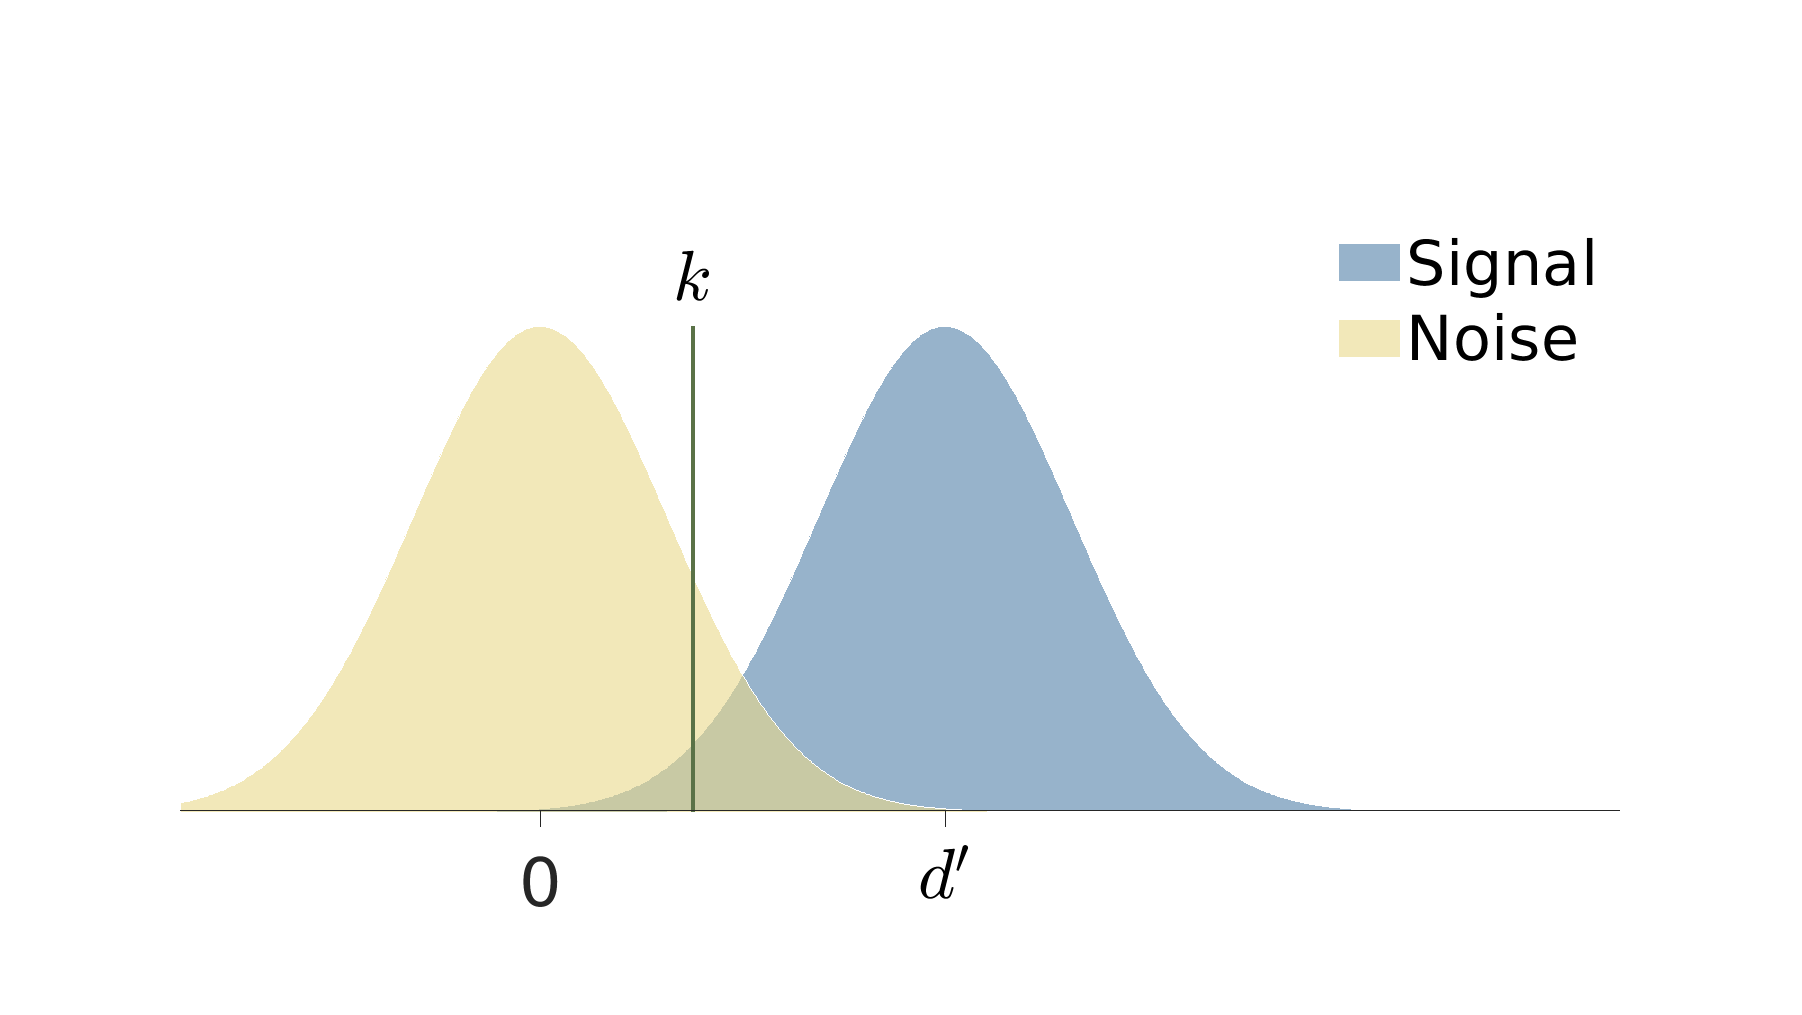
\includegraphics[width=\textwidth]{figures/signalDetectionTheory.pdf}
    \end{figure}
\end{frame}

\begin{frame}{Standard Model: Parameters}
  \frametitle{SDT: Model Parameters ($d'$, $c$)}
  Key parameters under standard assumptions:
  \begin{itemize}
    \item \textbf{Sensitivity ($\sdtDprime$):} Standardized difference between means.
      $$ \sdtDprime = \frac{\sdtMuSN - \sdtMuN}{\sdtSigma} $$
    \\[1ex]
      Measures distribution separation (signal-to-noise ratio).
    \pause
    \item \textbf{Criterion ($\sdtCrit$):} Position relative to the midpoint between means.
    $$ \sdtCrit = \frac{\sdtLambda - (\sdtMuN + \sdtMuSN)/2}{\sdtSigma} $$
    \\[1ex]
      Reflects response bias:
      \begin{itemize}
          \item $\sdtCrit=0$: Neutral bias (relative to midpoint).
          \item $\sdtCrit>0$: Conservative bias (need more evidence for ``Yes'').
          \item $\sdtCrit<0$: Liberal bias (need less evidence for ``Yes'').
      \end{itemize}
    \end{itemize}
\end{frame}

\begin{frame}{Standard Model: Parameters}
    \frametitle{SDT: Model Parameters ($d'$, $c$)}
    \begin{itemize}
    \item \textbf{Convention:} Often set $\sdtMuN = 0$ and $\sdtSigma = 1$. Then:
    \\[1ex]
      $ \qquad \text{Noise} \sim \mathcal{N}(0, 1) $
    \\[1ex]
      $ \qquad \text{Signal} \sim \mathcal{N}(\sdtDprime, 1) $
    \\[1ex]
      $ \qquad \sdtCrit = \sdtLambda - \sdtDprime/2 $
    \\[1ex]
      $ \qquad \sdtLambda = \sdtCrit + \sdtDprime/2 $ (Absolute criterion location)
  \end{itemize}
\end{frame}

\begin{frame}{Probabilities are areas}
    \begin{figure}
        \centering
        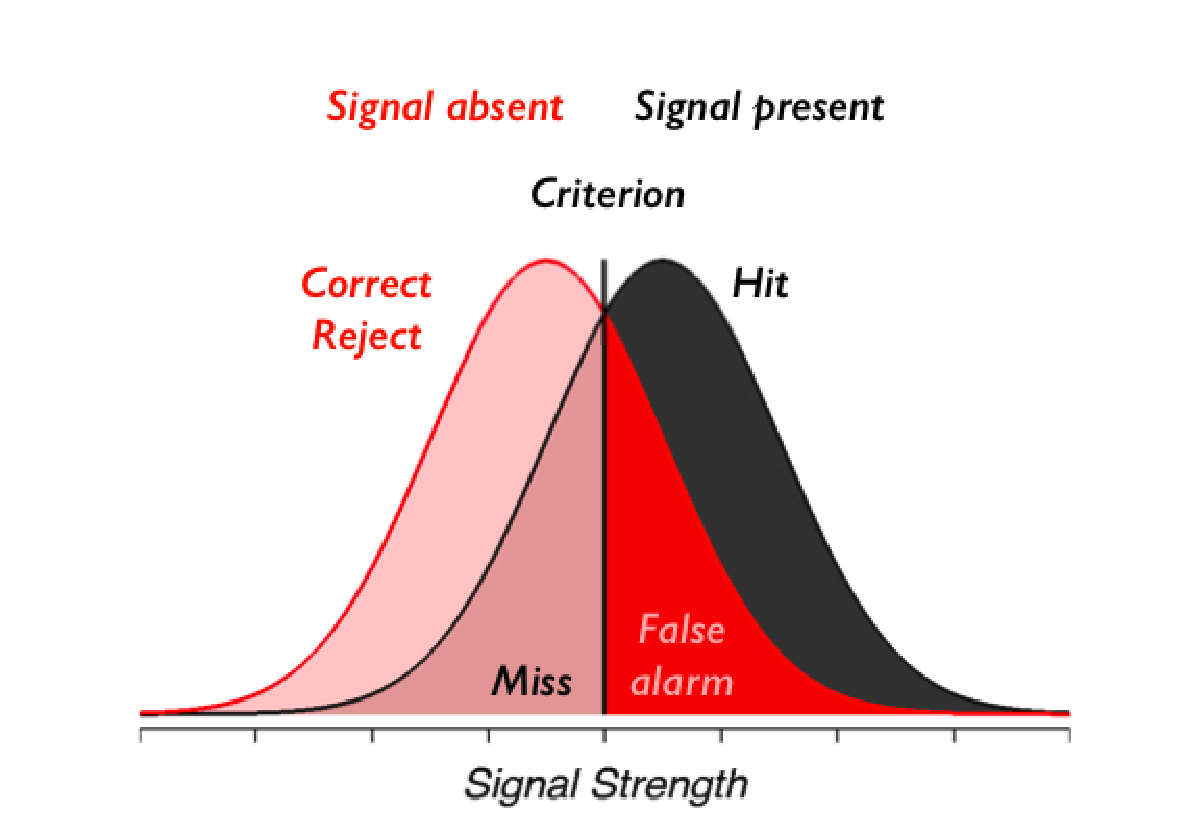
\includegraphics[width=.75\textwidth]{figures/area.pdf}
    \end{figure}
\end{frame}

\begin{frame}{Relating Parameters to Data}
  \frametitle{SDT: Linking Model to Data (HR, FAR)}
  The model links latent parameters ($\sdtDprime, \sdtCrit$) to observable data via Hit Rate (HR) and False Alarm Rate (FAR), using the standard normal CDF $\normalCDF{z} = P(Z \le z)$:
  \pause
  \begin{itemize}
    \item \textbf{Hit Rate (HR):} $P(\text{"Yes"} | \text{Signal})$
    \begin{align*}
      HR &= P(\text{Evidence} > \sdtLambda | \text{Signal}) \\
         &= P(Z > \frac{\sdtLambda - \sdtMuSN}{\sdtSigma}) \quad \text{(Standardize)}\\
         &= P(Z > \sdtLambda - \sdtDprime) \quad \text{(Using convention $\sdtMuSN=\sdtDprime, \sdtSigma=1$)}\\
         &= 1 - \normalCDF{\sdtLambda - \sdtDprime} = \normalCDF{\sdtDprime - \sdtLambda} \\
         &= \normalCDF{\sdtDprime - (\sdtCrit + \sdtDprime/2)} = \normalCDF{\sdtDprime/2 - \sdtCrit}
    \end{align*}
  \end{itemize}
\end{frame}


\begin{frame}{Relating Parameters to Data}
    \frametitle{SDT: Linking Model to Data (HR, FAR)}
    The model links latent parameters ($\sdtDprime, \sdtCrit$) to observable data via Hit Rate (HR) and False Alarm Rate (FAR), using the standard normal CDF $\normalCDF{z} = P(Z \le z)$:
    \begin{itemize}
      \item \textbf{False Alarm Rate (FAR):} $P(\text{"Yes"} | \text{Noise})$
      \begin{align*}
        FAR &= P(\text{Evidence} > \sdtLambda | \text{Noise}) \\
            &= P(Z > \frac{\sdtLambda - \sdtMuN}{\sdtSigma}) \quad \text{(Standardize)}\\
            &= P(Z > \sdtLambda) \quad \text{(Using convention $\sdtMuN=0, \sdtSigma=1$)}\\
            &= 1 - \normalCDF{\sdtLambda} = \normalCDF{-\sdtLambda} \\
            &= \normalCDF{-(\sdtCrit + \sdtDprime/2)} = \normalCDF{-\sdtDprime/2 - \sdtCrit}
      \end{align*}
    \end{itemize}
\end{frame}


\begin{frame}{Estimating Parameters from Data}
  \frametitle{SDT: Calculating $\sdtDprime$ and $\sdtCrit$}
  Equations can be inverted to estimate $\sdtDprime$ and $\sdtCrit$ from observed HR and FAR.
  \pause
  Let $z(p) = \invNormalCDF{p}$ be the inverse standard normal CDF (z-score or quantile function).
  \pause

  From:
  \begin{itemize}
      \item $HR = \normalCDF{\sdtDprime/2 - \sdtCrit} \implies \invNormalCDF{HR} = \sdtDprime/2 - \sdtCrit$
      \item $FAR = \normalCDF{-\sdtDprime/2 - \sdtCrit} \implies \invNormalCDF{FAR} = -\sdtDprime/2 - \sdtCrit$
  \end{itemize}
  \pause
  Solving this system yields:
  \\[2ex]
  $ \qquad \sdtDprime = \invNormalCDF{HR} - \invNormalCDF{FAR} $
  \\[2ex]
  $ \qquad \sdtCrit = -\frac{1}{2} [\invNormalCDF{HR} + \invNormalCDF{FAR}] $
\end{frame}

\begin{frame}{ROC Curves}
  \frametitle{SDT: ROC Curves}
  \textbf{Receiver Operating Characteristic (ROC) Curve:}
  \begin{itemize}
    \item Plots HR vs. FAR.
    \item Each point represents a (HR, FAR) pair achievable for a fixed sensitivity ($\sdtDprime$) by varying the criterion ($\sdtCrit$).
    \item Illustrates the trade-off: Increasing HR means increasing FAR for a given $\sdtDprime$.
    \pause
    \item \textbf{Properties:}
    \begin{itemize}
      \item Diagonal (HR = FAR) $\implies$ Chance performance ($\sdtDprime = 0$).
      \item Bows towards upper-left corner (HR=1, FAR=0 = Perfect).
      \item Degree of bowing reflects sensitivity (higher $\sdtDprime$ curves closer to top-left).
    \end{itemize}
    \pause
    \item \textbf{Area Under the ROC Curve (AUC):}
    \begin{itemize}
      \item Non-parametric measure of sensitivity, independent of bias.
      \item AUC = 0.5 $\implies$ Chance.
      \item AUC = 1.0 $\implies$ Perfect.
      \item For equal-variance Gaussian model: $AUC = \normalCDF{\sdtDprime / \sqrt{2}}$.
    \end{itemize}
  \end{itemize}
\end{frame}

\begin{frame}{ROC Curve Illustration}
    \begin{figure}
        \centering
        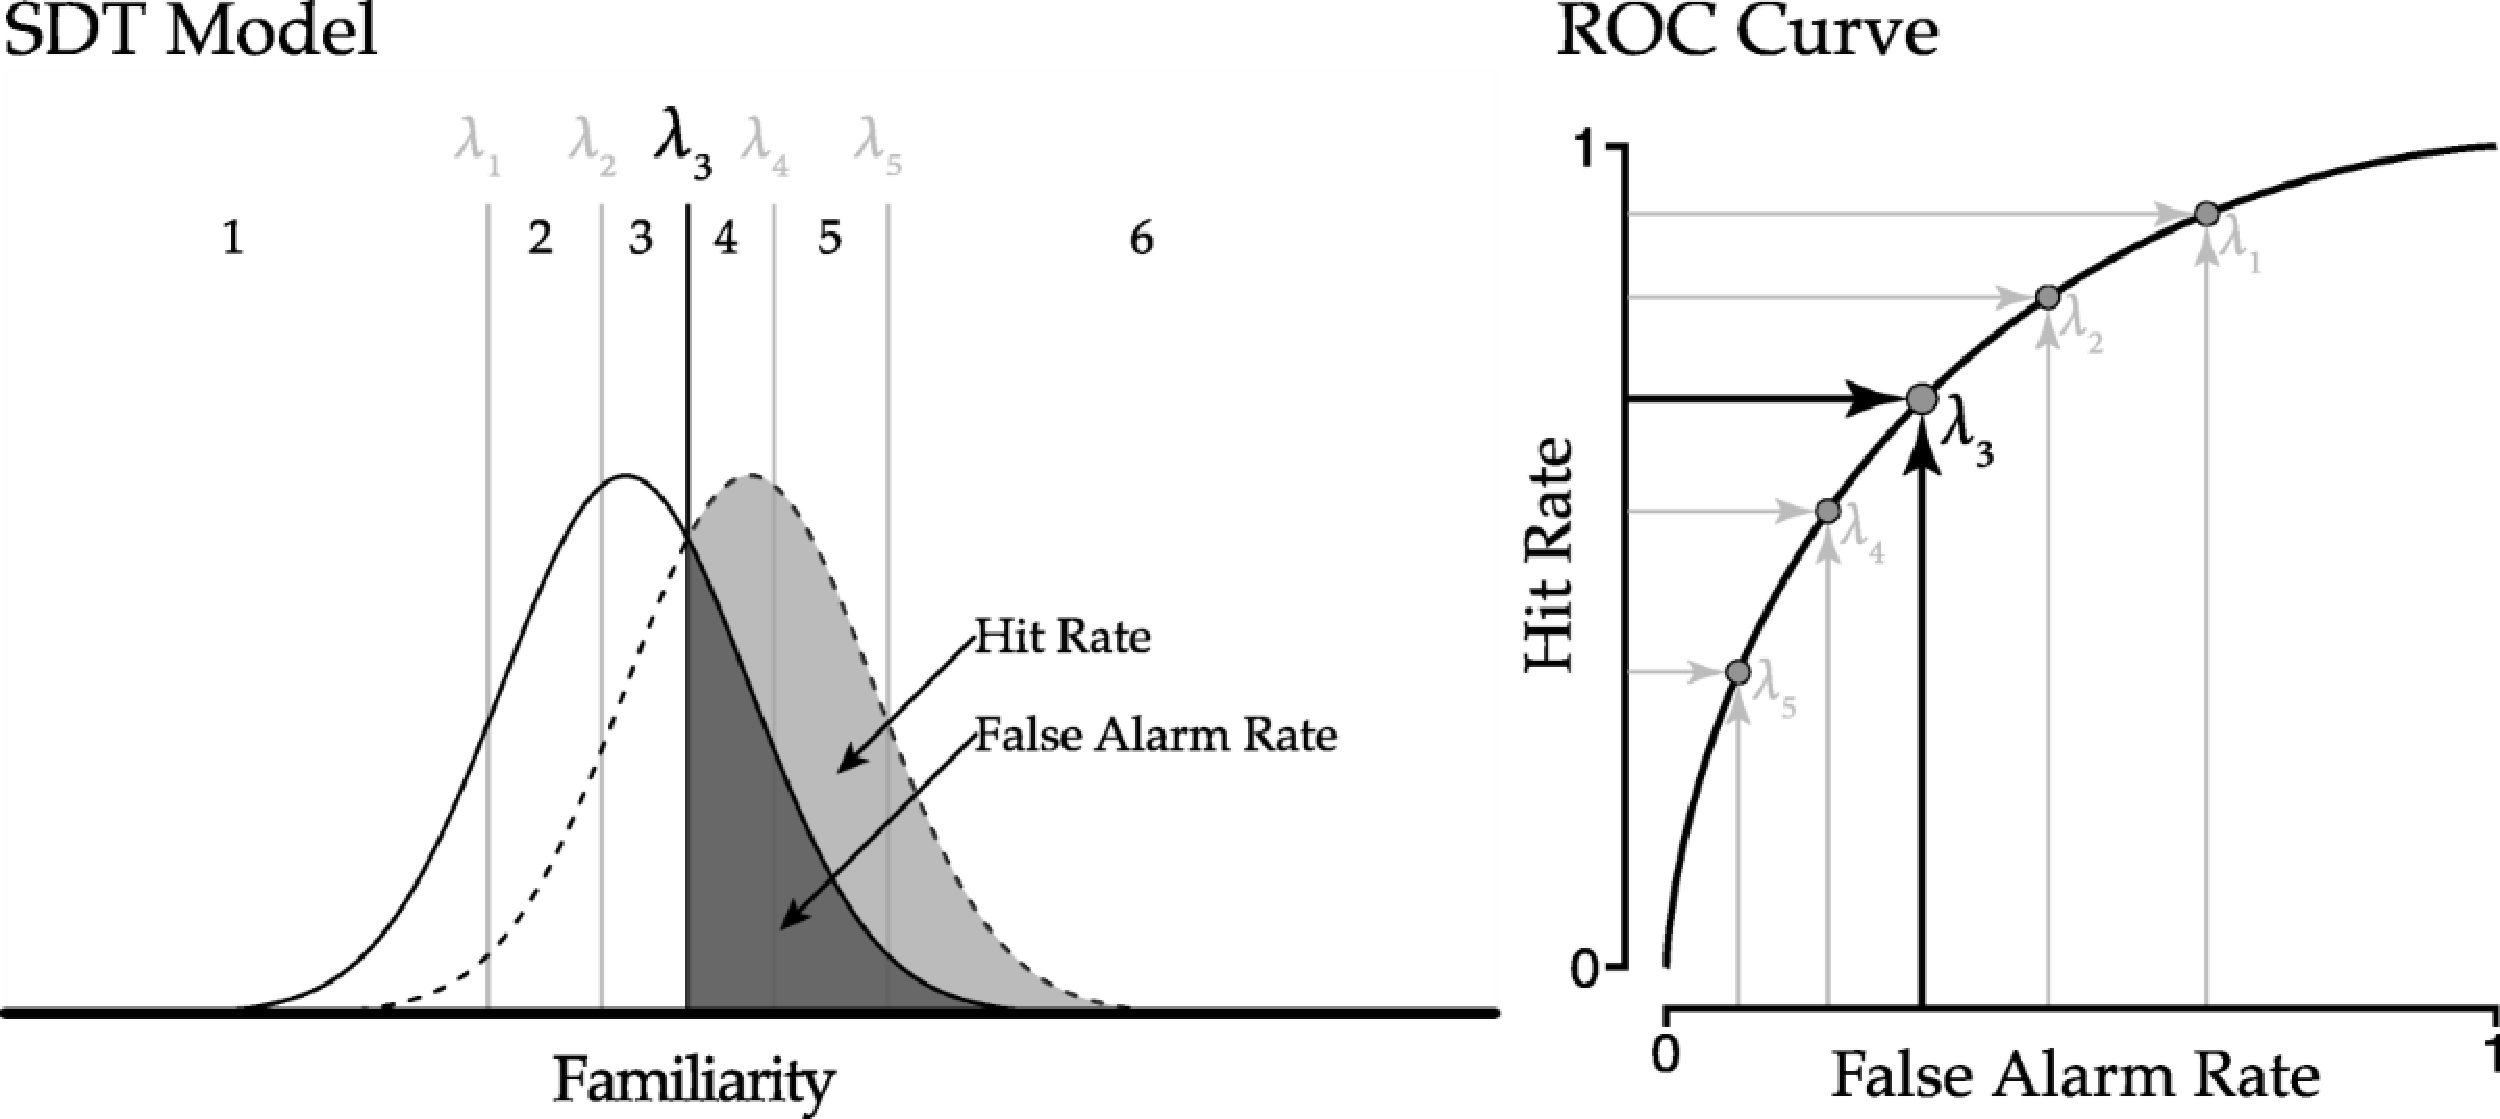
\includegraphics[width=\textwidth]{figures/basicroc.pdf}
    \end{figure}
\end{frame}


\begin{frame}{Assumptions, Extensions, Limitations}
  \frametitle{SDT: Assumptions \& Extensions}
  Standard model assumptions are often simplifications:
  \begin{itemize}
    \item \textbf{Unequal Variances (UVSDT):}
    \begin{itemize}
        \item Often more realistic, but harder to estimate (needs more data, e.g., ratings).
    \end{itemize}
    \item \textbf{Non-Gaussian Distributions:} Other evidence distributions (Poisson, Exponential) lead to different ROC shapes.
    \item \textbf{Criterion Variance:} Criterion might fluctuate across trials.
    \item \textbf{Task Dependence:} Model applies most directly to Yes/No tasks.
    \begin{itemize}
        \item \emph{Rating Scales:} Collect confidence ratings (e.g., 1-6). Allows plotting empirical ROC by collapsing ratings above different thresholds.
        \item \emph{Forced-Choice (e.g., 2AFC):} Choose interval/location with signal. Bias minimized. $PC = \normalCDF{\sdtDprime/\sqrt{2}}$ for 2AFC.
    \end{itemize}
  \end{itemize}
\end{frame}


\begin{frame}{Assumptions, Extensions, Limitations}
  \frametitle{SDT: Assumptions \& Extensions}
  \textbf{Limitations:} SDT is a descriptive, static model. It doesn't typically explain:
  \begin{itemize}
      \item Underlying mechanisms generating distributions.
      \item Time course of decision (see DDM, etc.).
      \item Dynamic changes (learning).
  \end{itemize}
\end{frame}

\begin{frame}{First assignment: PyMC Implementation}
  \frametitle{First assignment: PyMC Implementation (Basic SDT)}

  The concepts discussed in this lecture (estimating $d'$ and $c$ for one observer/condition) are implemented using PyMC in a Python script in the class repository:

  \begin{center}
    \texttt{0-introduction/src/sdt/basic.py}
  \end{center}

  This script demonstrates how to:
  \begin{itemize}
    \item Define priors for $d'$ and $c$.
    \item Link parameters to observed Hits and False Alarms using a Binomial likelihood.
    \item Sample from the posterior distribution using MCMC.
    \item Analyze and visualize the results (parameter estimates, uncertainty).
  \end{itemize}

  Your assignment is to start the class container and run this script. Then, explore the code to study a practical application of Bayesian SDT modeling for the basic case.
\end{frame}

\maketitle

\end{document} 